
%% bare_jrnl.tex
%% V1.3
%% 2007/01/11
%% by Michael Shell
%% see http://www.michaelshell.org/
%% for current contact information.
%%
%% This is a skeleton file demonstrating the use of IEEEtran.cls
%% (requires IEEEtran.cls version 1.7 or later) with an IEEE journal paper.
%%
%% Support sites:
%% http://www.michaelshell.org/tex/ieeetran/
%% http://www.ctan.org/tex-archive/macros/latex/contrib/IEEEtran/
%% and
%% http://www.ieee.org/



% *** Authors should verify (and, if needed, correct) their LaTeX system  ***
% *** with the testflow diagnostic prior to trusting their LaTeX platform ***
% *** with production work. IEEE's font choices can trigger bugs that do  ***
% *** not appear when using other class files.                            ***
% The testflow support page is at:
% http://www.michaelshell.org/tex/testflow/


%%*************************************************************************
%% Legal Notice:
%% This code is offered as-is without any warranty either expressed or
%% implied; without even the implied warranty of MERCHANTABILITY or
%% FITNESS FOR A PARTICULAR PURPOSE! 
%% User assumes all risk.
%% In no event shall IEEE or any contributor to this code be liable for
%% any damages or losses, including, but not limited to, incidental,
%% consequential, or any other damages, resulting from the use or misuse
%% of any information contained here.
%%
%% All comments are the opinions of their respective authors and are not
%% necessarily endorsed by the IEEE.
%%
%% This work is distributed under the LaTeX Project Public License (LPPL)
%% ( http://www.latex-project.org/ ) version 1.3, and may be freely used,
%% distributed and modified. A copy of the LPPL, version 1.3, is included
%% in the base LaTeX documentation of all distributions of LaTeX released
%% 2003/12/01 or later.
%% Retain all contribution notices and credits.
%% ** Modified files should be clearly indicated as such, including  **
%% ** renaming them and changing author support contact information. **
%%
%% File list of work: IEEEtran.cls, IEEEtran_HOWTO.pdf, bare_adv.tex,
%%                    bare_conf.tex, bare_jrnl.tex, bare_jrnl_compsoc.tex
%%*************************************************************************

% Note that the a4paper option is mainly intended so that authors in
% countries using A4 can easily print to A4 and see how their papers will
% look in print - the typesetting of the document will not typically be
% affected with changes in paper size (but the bottom and side margins will).
% Use the testflow package mentioned above to verify correct handling of
% both paper sizes by the user's LaTeX system.
%
% Also note that the "draftcls" or "draftclsnofoot", not "draft", option
% should be used if it is desired that the figures are to be displayed in
% draft mode.
%
\documentclass[journal]{IEEEtran}
\newtheorem{definition}{Definition}
\newtheorem{proposition}{Proposition} 
\newtheorem{remark}{Remark} 
%
% If IEEEtran.cls has not been installed into the LaTeX system files,
% manually specify the path to it like:
% \documentclass[journal]{../sty/IEEEtran}





% Some very useful LaTeX packages include:
% (uncomment the ones you want to load)


% *** MISC UTILITY PACKAGES ***
%
%\usepackage{ifpdf}
% Heiko Oberdiek's ifpdf.sty is very useful if you need conditional
% compilation based on whether the output is pdf or dvi.
% usage:
% \ifpdf
%   % pdf code
% \else
%   % dvi code
% \fi
% The latest version of ifpdf.sty can be obtained from:
% http://www.ctan.org/tex-archive/macros/latex/contrib/oberdiek/
% Also, note that IEEEtran.cls V1.7 and later provides a builtin
% \ifCLASSINFOpdf conditional that works the same way.
% When switching from latex to pdflatex and vice-versa, the compiler may
% have to be run twice to clear warning/error messages.






% *** CITATION PACKAGES ***
%
%\usepackage{cite}
% cite.sty was written by Donald Arseneau
% V1.6 and later of IEEEtran pre-defines the format of the cite.sty package
% \cite{} output to follow that of IEEE. Loading the cite package will
% result in citation numbers being automatically sorted and properly
% "compressed/ranged". e.g., [1], [9], [2], [7], [5], [6] without using
% cite.sty will become [1], [2], [5]--[7], [9] using cite.sty. cite.sty's
% \cite will automatically add leading space, if needed. Use cite.sty's
% noadjust option (cite.sty V3.8 and later) if you want to turn this off.
% cite.sty is already installed on most LaTeX systems. Be sure and use
% version 4.0 (2003-05-27) and later if using hyperref.sty. cite.sty does
% not currently provide for hyperlinked citations.
% The latest version can be obtained at:
% http://www.ctan.org/tex-archive/macros/latex/contrib/cite/
% The documentation is contained in the cite.sty file itself.






% *** GRAPHICS RELATED PACKAGES ***
%
\ifCLASSINFOpdf
  % \usepackage[pdftex]{graphicx}
  % declare the path(s) where your graphic files are
  % \graphicspath{{../pdf/}{../jpeg/}}
  % and their extensions so you won't have to specify these with
  % every instance of \includegraphics
  % \DeclareGraphicsExtensions{.pdf,.jpeg,.png}
\else
  % or other class option (dvipsone, dvipdf, if not using dvips). graphicx
  % will default to the driver specified in the system graphics.cfg if no
  % driver is specified.
  \usepackage[dvips]{graphicx}
  % declare the path(s) where your graphic files are
  % \graphicspath{{../eps/}}
  % and their extensions so you won't have to specify these with
  % every instance of \includegraphics
  \DeclareGraphicsExtensions{.eps}
\fi
% graphicx was written by David Carlisle and Sebastian Rahtz. It is
% required if you want graphics, photos, etc. graphicx.sty is already
% installed on most LaTeX systems. The latest version and documentation can
% be obtained at: 
% http://www.ctan.org/tex-archive/macros/latex/required/graphics/
% Another good source of documentation is "Using Imported Graphics in
% LaTeX2e" by Keith Reckdahl which can be found as epslatex.ps or
% epslatex.pdf at: http://www.ctan.org/tex-archive/info/
%
% latex, and pdflatex in dvi mode, support graphics in encapsulated
% postscript (.eps) format. pdflatex in pdf mode supports graphics
% in .pdf, .jpeg, .png and .mps (metapost) formats. Users should ensure
% that all non-photo figures use a vector format (.eps, .pdf, .mps) and
% not a bitmapped formats (.jpeg, .png). IEEE frowns on bitmapped formats
% which can result in "jaggedy"/blurry rendering of lines and letters as
% well as large increases in file sizes.
%
% You can find documentation about the pdfTeX application at:
% http://www.tug.org/applications/pdftex





% *** MATH PACKAGES ***
%
\usepackage[cmex10]{amsmath}
% A popular package from the American Mathematical Society that provides
% many useful and powerful commands for dealing with mathematics. If using
% it, be sure to load this package with the cmex10 option to ensure that
% only type 1 fonts will utilized at all point sizes. Without this option,
% it is possible that some math symbols, particularly those within
% footnotes, will be rendered in bitmap form which will result in a
% document that can not be IEEE Xplore compliant!
%
% Also, note that the amsmath package sets \interdisplaylinepenalty to 10000
% thus preventing page breaks from occurring within multiline equations. Use:
%\interdisplaylinepenalty=2500
% after loading amsmath to restore such page breaks as IEEEtran.cls normally
% does. amsmath.sty is already installed on most LaTeX systems. The latest
% version and documentation can be obtained at:
% http://www.ctan.org/tex-archive/macros/latex/required/amslatex/math/

\usepackage{amssymb}
\usepackage{amsfonts}




% *** SPECIALIZED LIST PACKAGES ***
%
%\usepackage{algorithmic}
% algorithmic.sty was written by Peter Williams and Rogerio Brito.
% This package provides an algorithmic environment fo describing algorithms.
% You can use the algorithmic environment in-text or within a figure
% environment to provide for a floating algorithm. Do NOT use the algorithm
% floating environment provided by algorithm.sty (by the same authors) or
% algorithm2e.sty (by Christophe Fiorio) as IEEE does not use dedicated
% algorithm float types and packages that provide these will not provide
% correct IEEE style captions. The latest version and documentation of
% algorithmic.sty can be obtained at:
% http://www.ctan.org/tex-archive/macros/latex/contrib/algorithms/
% There is also a support site at:
% http://algorithms.berlios.de/index.html
% Also of interest may be the (relatively newer and more customizable)
% algorithmicx.sty package by Szasz Janos:
% http://www.ctan.org/tex-archive/macros/latex/contrib/algorithmicx/




% *** ALIGNMENT PACKAGES ***
%
%\usepackage{array}
% Frank Mittelbach's and David Carlisle's array.sty patches and improves
% the standard LaTeX2e array and tabular environments to provide better
% appearance and additional user controls. As the default LaTeX2e table
% generation code is lacking to the point of almost being broken with
% respect to the quality of the end results, all users are strongly
% advised to use an enhanced (at the very least that provided by array.sty)
% set of table tools. array.sty is already installed on most systems. The
% latest version and documentation can be obtained at:
% http://www.ctan.org/tex-archive/macros/latex/required/tools/


%\usepackage{mdwmath}
%\usepackage{mdwtab}
% Also highly recommended is Mark Wooding's extremely powerful MDW tools,
% especially mdwmath.sty and mdwtab.sty which are used to format equations
% and tables, respectively. The MDWtools set is already installed on most
% LaTeX systems. The lastest version and documentation is available at:
% http://www.ctan.org/tex-archive/macros/latex/contrib/mdwtools/


% IEEEtran contains the IEEEeqnarray family of commands that can be used to
% generate multiline equations as well as matrices, tables, etc., of high
% quality.


%\usepackage{eqparbox}
% Also of notable interest is Scott Pakin's eqparbox package for creating
% (automatically sized) equal width boxes - aka "natural width parboxes".
% Available at:
% http://www.ctan.org/tex-archive/macros/latex/contrib/eqparbox/





% *** SUBFIGURE PACKAGES ***
%\usepackage[tight,footnotesize]{subfigure}
% subfigure.sty was written by Steven Douglas Cochran. This package makes it
% easy to put subfigures in your figures. e.g., "Figure 1a and 1b". For IEEE
% work, it is a good idea to load it with the tight package option to reduce
% the amount of white space around the subfigures. subfigure.sty is already
% installed on most LaTeX systems. The latest version and documentation can
% be obtained at:
% http://www.ctan.org/tex-archive/obsolete/macros/latex/contrib/subfigure/
% subfigure.sty has been superceeded by subfig.sty.



%\usepackage[caption=false]{caption}
%\usepackage[font=footnotesize]{subfig}
% subfig.sty, also written by Steven Douglas Cochran, is the modern
% replacement for subfigure.sty. However, subfig.sty requires and
% automatically loads Axel Sommerfeldt's caption.sty which will override
% IEEEtran.cls handling of captions and this will result in nonIEEE style
% figure/table captions. To prevent this problem, be sure and preload
% caption.sty with its "caption=false" package option. This is will preserve
% IEEEtran.cls handing of captions. Version 1.3 (2005/06/28) and later 
% (recommended due to many improvements over 1.2) of subfig.sty supports
% the caption=false option directly:
%\usepackage[caption=false,font=footnotesize]{subfig}
%
% The latest version and documentation can be obtained at:
% http://www.ctan.org/tex-archive/macros/latex/contrib/subfig/
% The latest version and documentation of caption.sty can be obtained at:
% http://www.ctan.org/tex-archive/macros/latex/contrib/caption/




% *** FLOAT PACKAGES ***
%
%\usepackage{fixltx2e}
% fixltx2e, the successor to the earlier fix2col.sty, was written by
% Frank Mittelbach and David Carlisle. This package corrects a few problems
% in the LaTeX2e kernel, the most notable of which is that in current
% LaTeX2e releases, the ordering of single and double column floats is not
% guaranteed to be preserved. Thus, an unpatched LaTeX2e can allow a
% single column figure to be placed prior to an earlier double column
% figure. The latest version and documentation can be found at:
% http://www.ctan.org/tex-archive/macros/latex/base/



%\usepackage{stfloats}
% stfloats.sty was written by Sigitas Tolusis. This package gives LaTeX2e
% the ability to do double column floats at the bottom of the page as well
% as the top. (e.g., "\begin{figure*}[!b]" is not normally possible in
% LaTeX2e). It also provides a command:
%\fnbelowfloat
% to enable the placement of footnotes below bottom floats (the standard
% LaTeX2e kernel puts them above bottom floats). This is an invasive package
% which rewrites many portions of the LaTeX2e float routines. It may not work
% with other packages that modify the LaTeX2e float routines. The latest
% version and documentation can be obtained at:
% http://www.ctan.org/tex-archive/macros/latex/contrib/sttools/
% Documentation is contained in the stfloats.sty comments as well as in the
% presfull.pdf file. Do not use the stfloats baselinefloat ability as IEEE
% does not allow \baselineskip to stretch. Authors submitting work to the
% IEEE should note that IEEE rarely uses double column equations and
% that authors should try to avoid such use. Do not be tempted to use the
% cuted.sty or midfloat.sty packages (also by Sigitas Tolusis) as IEEE does
% not format its papers in such ways.


%\ifCLASSOPTIONcaptionsoff
%  \usepackage[nomarkers]{endfloat}
% \let\MYoriglatexcaption\caption
% \renewcommand{\caption}[2][\relax]{\MYoriglatexcaption[#2]{#2}}
%\fi
% endfloat.sty was written by James Darrell McCauley and Jeff Goldberg.
% This package may be useful when used in conjunction with IEEEtran.cls'
% captionsoff option. Some IEEE journals/societies require that submissions
% have lists of figures/tables at the end of the paper and that
% figures/tables without any captions are placed on a page by themselves at
% the end of the document. If needed, the draftcls IEEEtran class option or
% \CLASSINPUTbaselinestretch interface can be used to increase the line
% spacing as well. Be sure and use the nomarkers option of endfloat to
% prevent endfloat from "marking" where the figures would have been placed
% in the text. The two hack lines of code above are a slight modification of
% that suggested by in the endfloat docs (section 8.3.1) to ensure that
% the full captions always appear in the list of figures/tables - even if
% the user used the short optional argument of \caption[]{}.
% IEEE papers do not typically make use of \caption[]'s optional argument,
% so this should not be an issue. A similar trick can be used to disable
% captions of packages such as subfig.sty that lack options to turn off
% the subcaptions:
% For subfig.sty:
% \let\MYorigsubfloat\subfloat
% \renewcommand{\subfloat}[2][\relax]{\MYorigsubfloat[]{#2}}
% For subfigure.sty:
% \let\MYorigsubfigure\subfigure
% \renewcommand{\subfigure}[2][\relax]{\MYorigsubfigure[]{#2}}
% However, the above trick will not work if both optional arguments of
% the \subfloat/subfig command are used. Furthermore, there needs to be a
% description of each subfigure *somewhere* and endfloat does not add
% subfigure captions to its list of figures. Thus, the best approach is to
% avoid the use of subfigure captions (many IEEE journals avoid them anyway)
% and instead reference/explain all the subfigures within the main caption.
% The latest version of endfloat.sty and its documentation can obtained at:
% http://www.ctan.org/tex-archive/macros/latex/contrib/endfloat/
%
% The IEEEtran \ifCLASSOPTIONcaptionsoff conditional can also be used
% later in the document, say, to conditionally put the References on a 
% page by themselves.





% *** PDF, URL AND HYPERLINK PACKAGES ***
%
%\usepackage{url}
% url.sty was written by Donald Arseneau. It provides better support for
% handling and breaking URLs. url.sty is already installed on most LaTeX
% systems. The latest version can be obtained at:
% http://www.ctan.org/tex-archive/macros/latex/contrib/misc/
% Read the url.sty source comments for usage information. Basically,
% \url{my_url_here}.





% *** Do not adjust lengths that control margins, column widths, etc. ***
% *** Do not use packages that alter fonts (such as pslatex).         ***
% There should be no need to do such things with IEEEtran.cls V1.6 and later.
% (Unless specifically asked to do so by the journal or conference you plan
% to submit to, of course. )


% correct bad hyphenation here
\hyphenation{op-tical net-works semi-conduc-tor}


\begin{document}
%
% paper title
% can use linebreaks \\ within to get better formatting as desired
\title{On the Accommodation of a Large Number of Contenders in CSMA/ECA}
%
%
% author names and IEEE memberships
% note positions of commas and nonbreaking spaces ( ~ ) LaTeX will not break
% a structure at a ~ so this keeps an author's name from being broken across
% two lines.
% use \thanks{} to gain access to the first footnote area
% a separate \thanks must be used for each paragraph as LaTeX2e's \thanks
% was not built to handle multiple paragraphs
%

\author{Michael~Shell,~\IEEEmembership{Member,~IEEE,}
        John~Doe,~\IEEEmembership{Fellow,~OSA,}
        and~Jane~Doe,~\IEEEmembership{Life~Fellow,~IEEE}% <-this % stops a space
\thanks{M. Shell is with the Department
of Electrical and Computer Engineering, Georgia Institute of Technology, Atlanta,
GA, 30332 USA e-mail: (see http://www.michaelshell.org/contact.html).}% <-this % stops a space
\thanks{J. Doe and J. Doe are with Anonymous University.}% <-this % stops a space
\thanks{Manuscript received April 19, 2005; revised January 11, 2007.}}

% note the % following the last \IEEEmembership and also \thanks - 
% these prevent an unwanted space from occurring between the last author name
% and the end of the author line. i.e., if you had this:
% 
% \author{....lastname \thanks{...} \thanks{...} }
%                     ^------------^------------^----Do not want these spaces!
%
% a space would be appended to the last name and could cause every name on that
% line to be shifted left slightly. This is one of those "LaTeX things". For
% instance, "\textbf{A} \textbf{B}" will typeset as "A B" not "AB". To get
% "AB" then you have to do: "\textbf{A}\textbf{B}"
% \thanks is no different in this regard, so shield the last } of each \thanks
% that ends a line with a % and do not let a space in before the next \thanks.
% Spaces after \IEEEmembership other than the last one are OK (and needed) as
% you are supposed to have spaces between the names. For what it is worth,
% this is a minor point as most people would not even notice if the said evil
% space somehow managed to creep in.



% The paper headers
\markboth{Journal of \LaTeX\ Class Files,~Vol.~6, No.~1, January~2007}%
{Shell \MakeLowercase{\textit{et al.}}: Bare Demo of IEEEtran.cls for Journals}
% The only time the second header will appear is for the odd numbered pages
% after the title page when using the twoside option.
% 
% *** Note that you probably will NOT want to include the author's ***
% *** name in the headers of peer review papers.                   ***
% You can use \ifCLASSOPTIONpeerreview for conditional compilation here if
% you desire.




% If you want to put a publisher's ID mark on the page you can do it like
% this:
%\IEEEpubid{0000--0000/00\$00.00~\copyright~2007 IEEE}
% Remember, if you use this you must call \IEEEpubidadjcol in the second
% column for its text to clear the IEEEpubid mark.



% use for special paper notices
%\IEEEspecialpapernotice{(Invited Paper)}




% make the title area
\maketitle


\begin{abstract}
%\boldmath
In this paper we use a Markov Chain to model a simple solver for Decentralized Constrain Satisfaction problems.
We provide closed expressions to compute the transition probabilities and the transition probabilities matrix can then be used to determine the expected number of steps that the system requires to converge to a solution.
We use a protocol to allocate channel slots to contending stations as an illustrating example, and extend our model to contemplate the possibility of channel errors.
The model is validated by means of simulation and we show that it can be easily extended to account for the presence of errors.
\end{abstract}
% IEEEtran.cls defaults to using nonbold math in the Abstract.
% This preserves the distinction between vectors and scalars. However,
% if the journal you are submitting to favors bold math in the abstract,
% then you can use LaTeX's standard command \boldmath at the very start
% of the abstract to achieve this. Many IEEE journals frown on math
% in the abstract anyway.

% Note that keywords are not normally used for peerreview papers.
\begin{IEEEkeywords}
Decentralized constraint satisfaction, Markov Chain model, collision-free operation, medium access control
\end{IEEEkeywords}






% For peer review papers, you can put extra information on the cover
% page as needed:
% \ifCLASSOPTIONpeerreview
% \begin{center} \bfseries EDICS Category: 3-BBND \end{center}
% \fi
%
% For peerreview papers, this IEEEtran command inserts a page break and
% creates the second title. It will be ignored for other modes.
\IEEEpeerreviewmaketitle



\section{Introduction}
% The very first letter is a 2 line initial drop letter followed
% by the rest of the first word in caps.
% 
% form to use if the first word consists of a single letter:
% \IEEEPARstart{A}{demo} file is ....
% 
% form to use if you need the single drop letter followed by
% normal text (unknown if ever used by IEEE):
% \IEEEPARstart{A}{}demo file is ....
% 
% Some journals put the first two words in caps:
% \IEEEPARstart{T}{his demo} file is ....
% 
% Here we have the typical use of a "T" for an initial drop letter
% and "HIS" in caps to complete the first word.
\IEEEPARstart{T}{his} demo file is intended to serve as a ``starter file''
for IEEE journal papers produced under \LaTeX\ using
IEEEtran.cls version 1.7 and later.
% You must have at least 2 lines in the paragraph with the drop letter
% (should never be an issue)


\section{Introduction}

In this paper we introduce a Markov Chain (MC) model that captures the convergence process of a solver for Decentralized Constraint Satisfaction (DCS) problems.
DCS problems can be used to distributively allocate radio resources to competing wireless stations.
As DCS work iteratively, stochastically searching for a solution, it is necessary to gain some insight on the convergence process and estimate the number of steps required to reach a solution.

DCS problems and solvers are introduced in Sect. \ref{sec:dcs}, together with examples of practical applications.
The model is described in Sect. \ref{sec:markov_chain} and numerical results are presented in Sect.~\ref{sec:numerical_results}.
Finally, Sect.~\ref{sec:conclusion} concludes the paper.

\section{Related Work}
Since the inception of wireless local area networks (WLANs), random medium access mechanisms have played a key role to arbitrate the access to the channel.
The core principles of the medium access control (MAC) that were introduced in the first release of the IEEE 802.11 standard are still valid today \cite{IEEE80211-IEEESTD2007}.
The contending stations use carrier sense to prevent that a station interrupts another transmission.
Slotted time combined with a backoff counter is used to reduce the chances that two stations simultaneously start a transmission.
Until today, this backoff counter has been initialized with a random value.
Stations separate two transmission attempts by a random backoff, to give the opportunity to other stations to transmit.

Recently, it has been pointed out that the random choice of the backoff value is not necessary after successful transmissions \cite{barcelo2008lba}.
In fact, if the backoff value is deterministically chosen after successful transmissions, the chances of collisions are reduced.
Furthermore, under certain idealistic conditions, the collision-free operation can be reached.
The idea of using a deterministic backoff after successful transmissions has been later explored in more detail in, e.g, \cite{he2009srb,barcelo2011tcf,fang2011dlm}.

It is possible to model a protocol in which a deterministic backoff is used after successful collisions and a random backoff otherwise as a Markov Chain \cite{he2009srb, barcelo2010fcc}.
This model is just a mathematically amenable approximation of the actual protocols.
We will describe this model in the next section, and it will be used as a reference protocol for the rest of the paper.

The problem that is addressed by this protocol is the decentralized assignment of stations to slots in such a way that there is no slot that contains more than one stations.
Nevertheless, similar problems can be found in other areas of networking.
Examples are provided in \cite{duffy2011dcs}, that accurately defines this family of problems and names it \emph{Decentralized Constraint Satisfaction} (DCS).
The same paper also describes a solver and characterizes it by providing a bound that describes the convergence properties of the solver.

In the present paper, we will consider a particular instance of that solver and compute the expected number of rounds that are required by the solver to find the solution.

We will use the convention to say that a slot is successful when there is a single station transmitting in that slot.
Similarly, we will refer to the station transmitting in the successful slot as a successful station.
In our analysis, we will be presented with the problem of counting the number of successful slots when $N$ stations choose among $B$ slots.
The particular case in which all the stations randomly choose the transmission slot has already been addressed in the literature in \cite{szpankowski1983asc}.
However, in the present paper, we have to consider also the case in which some of the stations choose their transmission slot deterministically while the remaining stations randomly choose their transmission slot.


\section{Decentralized Constraint Satisfaction}
\label{sec:dcs}
The analytical model we present in this paper describes what is defined as a Decentralized Constraint Satisfaction problem. A Constraint Satisfaction problem with $N$ variables is defined as follows (adopting the notation from \cite{duffy2011dcs}).
We consider $N$ variables,  \mbox{$\mathbf{x} := (x_1,\dots,x_N)$}, each one taking values in a finite set $\mathbf{B}=\left\{1, \dots, B \right\} \subset \mathbb{N} $.
We consider also $M$ clauses that are boolean functions, $\left\{ \Phi_1(\mathbf{x}),\dots,\Phi_M(\mathbf{x}) \right\}$.
These $M$ clauses represent the constraints and take a value equal to 1 if the constrained is satisfied and 0 otherwise.
An assignment $\mathbf{x}$ is a solution to the problem if all the constraints are satisfied.
While there are solvers for this kind of problem, they are typically centralized, i.e., assuming that the solver has the complete information about all variables. 
In the reality of data networks in particular, this assumption normally does not hold. Examples typically can be found in the area of wireless networks, e.g., wireless sensor or mesh networks. 

Here, the variables can be interpreted as the channel chosen by a device in a shared medium. This channel may for example be a frequency or a time slot. The clauses then evaluate if two or more stations chose the same channel (in which case, collisions occur), or all have selected their own channel (the desired situation). 

No communication can occur between the endpoints trying to solve the Constraint Satisfaction Problem, since the problem is to establish a collision-free communication in the first place. Therefore, we are here considering a special case, namely a DCS problem. Essentially, this means that any device sharing the medium only can control one variable, namely its channel selection, and only has information about the clauses including this variable, namely whether a collision occurred or not.

To illustrate this, we will shortly cover two examples. The first is a set of WLAN access points, which need to select the channels they use in a distributed fashion. Since access points too close to each other may interfere with each other's communication, but may not be able to communicate directly with each other, this presents a DCS problem, with the set of different channels to choose from at each access point being the variable, the number of variables being the number of access points considered, and the clauses describing, for every pair of access points in interference range, whether they have selected the same channel or not.

As a second example, we consider carrier sense multiple access with collision avoidance (CSMA/CA). Here, a contending station with a packet to transmit defers its transmission for a random number of slots if the (shared) channel is sensed busy.
This protocol reduces the likelihood of collisions as a collision happens only when two or more contending stations select the same slot for transmission.
The operation of the protocol is illustrated in Fig.~\ref{fig:csma_ca_compact}.

\begin{figure}
  \centering
  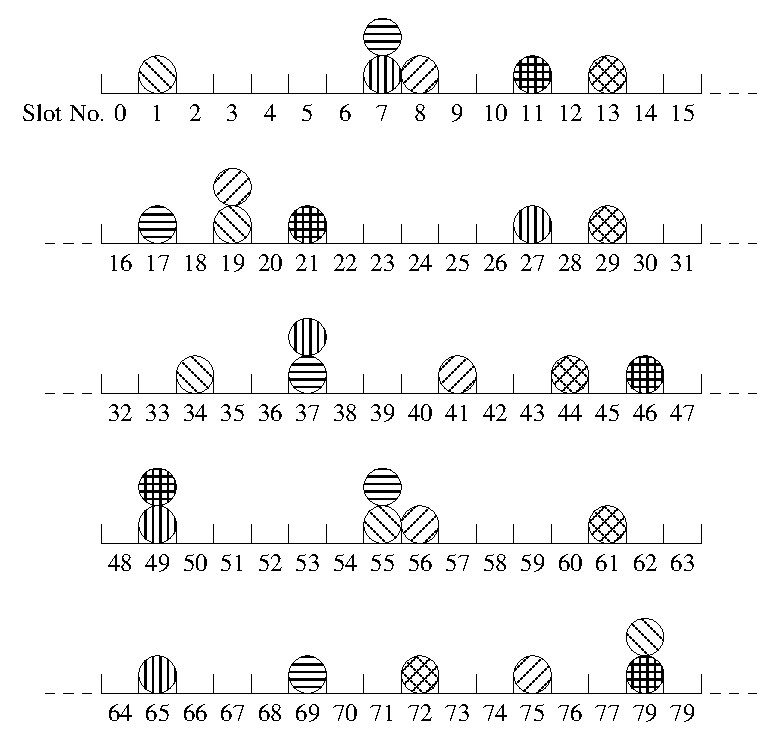
\includegraphics[width=2.5in]{figures/csma_ca_compact}
  \caption{CSMA/CA contention}
  \label{fig:csma_ca_compact}
\end{figure}
\begin{figure}
  \centering
  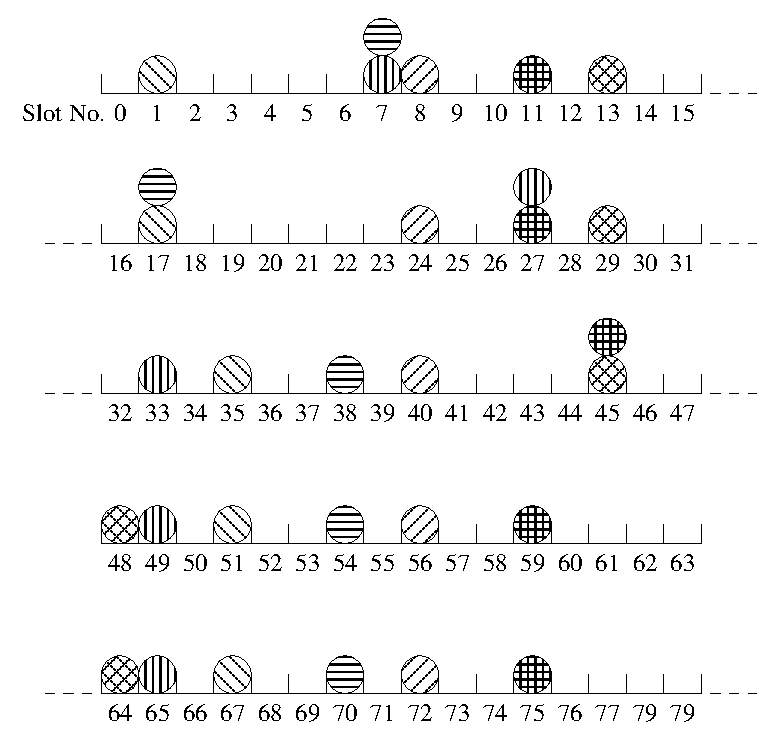
\includegraphics[width=2.5in]{figures/csma_eca_compact}
  \caption{CSMA/ECA contention}
  \label{fig:csma_eca_compact}
\end{figure}

CSMA/CA can be improved if the participating stations defer the transmission for a deterministic backoff after successful transmissions.
This approach is represented in Fig.~\ref{fig:csma_eca_compact}.
The variant of the protocol that uses a deterministic backoff after successful transmissions is called CSMA with enhanced collision avoidance (CSMA/ECA).
A more detailed explanation of CSMA/ECA can be found in, e.g., \cite{barcelo2008lba,barcelo2009tpc,he2009srb,fang2011dlm}.

For this example, the values of the variables in the according DCS problem are the different slots to choose from, while the number of variables is the number of stations sharing the channel. The clauses are again evaluating, for each pair of variables, if they have the same value or not.
This is equivalent to check if two stations have selected the same slot for transmission.

For these problems, a DCS solver has been presented in \cite{duffy2011dcs}. The contribution of this paper is to present an analytical model based on a MC that describes the behavior of this solver in a specific case, as described in the next section.

\section{The Markov Chain Model}
\label{sec:markov_chain}

The solver developed in \cite{duffy2011dcs} uses two parameters $a$ and $b$, that we set to one. With this parametrization, the behavior of the solver is extremely simple.
In a first step, the variables $x_i$ are assigned a value randomly. Then the constraints are evaluated.
Those variables that are involved in constraints that are not satisfied take a random value in the next step, while the other variables keep the same value as in the previous step.
When the solution is reached, all the variables keep the same value.
This is, e.g., roughly equivalent to the CSMA/ECA protocol described in the previous section.
In the protocol, when all the stations successfully transmit, a collision-free schedule has been reached that it is repeated in the following rounds.

To analyze this behavior, standard MC theory can be used to estimate the expected number of steps required to reach the solution. To illustrate the solution better, we will use the protocol described in the previous paragraph as the on-going example.

For this contention protocol, considering that we have $N$ contending stations, the associated MC model has $N+1$ different states, $S_0, \dots, S_N$.
The system is in state $S_d$ if exactly $d$ stations ($0 \leq d \leq N$) will deterministically chose their transmission slot in the next round.
From the constraint satisfaction problem perspective, this is equivalent to saying that there are $d$ variables that are not involved in constraints that are not satisfied.
We are interested in the computation of the transition probabilities from one state $S_d$ to another state $S_\delta$, $0 \leq \delta \leq N$.
We formalize this transition probability in the following definition.

\begin{definition}
For given values of $B$ and $N$, let us define $\psi_{d,\delta}^{B,N}$ as the transition probability from $S_d$ to $S_\delta$. 
\end{definition}

This $\psi_{d,\delta}^{B,N}$ is the probability of obtaining $\delta$ successful transmissions given $N$ stations and $B$ slots when $d$ of the stations use a deterministically chosen slot while the remaining $N-d$ stations transmit in a randomly chosen slot.

\begin{remark}
The considered MC is an absorbing MC, as $\psi_{d,\delta}^{B,N}=1$ when both $d$ and $\delta$ are equal to $N$.
\end{remark}

Once a collision-free schedule is found, the same collision-free schedule is repeated in every subsequent step.
Since the MC is absorbing, the expected number of steps before convergence can be computed if the values of $\psi_{d,\delta}^{B,N}$ are known \cite{grinstead1997ip}.

Later in the article we will provide a formula to compute $\psi_{d,\delta}^{B,N}$.
As first step, we analyze the simpler case in which $d=0$, which means that all the stations are randomly choosing their transmission slot. 
This particular case is considered in Proposition \ref{pro:zero_case}.

\begin{proposition}
\label{pro:zero_case}
The probability $\psi^{B,N}_{d,\delta}$ in the particular case when $d=0$ is 
\setlength{\arraycolsep}{0.0em}
\begin{eqnarray}
\psi^{B,N}_{0,\delta} & {}={} &\sum_{j=\delta}^{N-1} (-1)^{j+\delta}\binom{j}{\delta} \binom{N}{j}\frac{B! (B-j)^{N-j}}{(B-j)! B^N} \nonumber\\
&&{+}\:(-1)^{N+\delta}\binom{N}{\delta}\frac{B!}{(B-N)!B^N}
\label{eq:psi_zero}
\end{eqnarray}
\end{proposition}

\begin{proof}
We are considering transitions from the state $S_0$ in which all the stations behave randomly to the other states. 
Our aim is to compute the transition probabilities from $S_0$ to another state $S_\delta$, $0\leq \delta \leq N$, which is the probability that exactly $\delta$ stations successfully transmit.
Some intermediate steps are necessary to compute the transition probabilities.

We will define a set of $N$ events which represent the success of each of the $N$ stations and then we consider intersections among these events.
As an example, to compute the transition from $S_0$ to $S_1$ we need to compute the probability that exactly one of the stations successfully transmits.
This is a counting problem in which we need to count all the cases in which exactly one of the stations successfully transmit.
We will use a theorem that addresses this specific problem as we detail in the Appendix.

We number the stations from $1$ to $N$ for convenience, and we define $A_i$, ($i=1,\cdots,N$) the event that station $i$ succeeds and $\mathbf{A}=\{A_i:i=1,\dots,N\}$ the collection of these events.
Notice that these events are partially overlapping, since it is possible that more than one station successfully transmits.

We derive the probability of the event $A_i$ ($i=1\dots N$) as follows:
the probability that a tagged stations succeeds is simply the probability that the remaining $N-1$ stations choose a different slot from the tagged station.
As there are a total of $B-1$ of such slots, the probability that all $N-1$ stations choose among those $B-1$ slots out of the total $B$ slots is given by
\begin{equation}
P(A_i)=\left(\frac{B-1}{B} \right)^{N-1}.
\end{equation}

In the following, we will derive the probability that a selection of $j$ tagged stations succeeds.
Let $\mathbf{A}^j$ be a set of $j$ ($j\leq N$) events in $\mathbf{A}$, that is $\mathbf{A}^j \subseteq \mathbf{A}, |\mathbf{A}^j|=j$.
Without loss of generality, and to clarify the explanation, we take the ordered list of the tagged stations and assume that they choose, one by one, from 1 to $j$, the slot in which they transmit. 
The first tagged station chooses any slot.
The second station chooses any slot different from the one chosen by the first one with probability $(B-1)/B$. 
In general, the $l$-th ($1 \leq l \leq j$) tagged station chooses one of the remaining slots with probability $(B-(l-1))/B$.
Finally, we need that the remaining $N-j$ non tagged stations (if any) choose the slots that are not occupied by the tagged stations, which occurs with probability $\left( \frac{B-j}{B}\right)^{N-j}$.

Summing up, for $1 \leq j \leq N-1$ the probability that all the $j$ tagged stations successfully transmit is given by
\begin{equation}
\label{eq:prob_j_sta_transmit}
P\left( A_\cap \right) = \frac{B}{B} \cdot \frac{B-1}{B} \cdot \dots \cdot \frac{B-(j-1)}{B} \cdot \left( \frac{B-j}{B} \right)^{N-j},
\end{equation}
where $A_\cap=\bigcap_{ A_i \in \mathbf{A}^j}A_i$ and $j=1\dots N-1$.

Rewriting (\ref{eq:prob_j_sta_transmit}), we obtain
\begin{equation}
\label{eq:PA}
P\left( A_\cap \right) = \frac{B! (B-j)^{N-j}}{(B-j)! B^N},
\quad j=1\dots N-1.
\end{equation}

Now, let us define $S(0,j)$ as the sum of the probabilities of occurrence of all the $\binom{N}{j}$ subsets $\mathbf{A}^j$ of size $|\mathbf{A}^j|=j$. For $j < N$ it is, 

\begin{eqnarray}
\label{eq:S0j}
S(0,j) & {}={}  & \sum_{\scriptstyle \mathbf{A}^j\subseteq\mathbf{A}} P\left( A_\cap \right) \\
&{}={}& \sum_{\scriptstyle \mathbf{A}^j\subseteq\mathbf{A}} \binom{N}{j}\frac{B! (B-j)^{N-j}}{(B-j)! B^N},
\quad j=1 \dots N-1. \nonumber
\end{eqnarray}

The expressions for (\ref{eq:PA}) and (\ref{eq:S0j}) in the case that all the stations succeed ($j=N$) are:
\begin{equation}
P\left( \bigcap_{ A_i \in \mathbf{A}^N } A_i \right) = \frac{B!}{(B-N)! B^N}
,
\end{equation}

and
\begin{equation}
S(0,N)=\sum_{\scriptstyle \mathbf{A}^N\subseteq\mathbf{A}} P\biggl(\bigcap_{A_i\in \mathbf{A}^N} A_i \biggr) 
=\frac{B!}{(B-N)! B^N}.
\end{equation}



Finally, we will derive the value of $\psi_{0,n}^{B,N}$ applying the theorem in Sec. IV.3 of \cite{feller1968ipt} as exemplified in the Appendix.
The result is:

\begin{equation}
\begin{split}
\psi^{B,N}_{0,\delta} = \sum_{j=\delta}^{N} (-1)^{j+\delta}\binom{j}{\delta} S(0,j)= \\
\sum_{j=\delta}^{N-1} (-1)^{j+\delta}\binom{j}{\delta} \binom{N}{j}\frac{B! (B-j)^{N-j}}{(B-j)! B^N}
+ (-1)^{N+\delta}\binom{N}{\delta}\frac{B!}{(B-N)! B^N}.
\end{split}
\label{eq:psi_zero}
\end{equation}


\end{proof}

\begin{proposition}
\label{pro:general_case}
The probability $\psi^{B,N}_{d,\delta}$ is 
\begin{equation}
\begin{split}
\psi^{B,N}_{d,\delta} = \\
\sum_{j=\delta}^{N-1} (-1)^{j+\delta} \binom{j}{\delta} 
\sum_{i=max(0,j+d-N)}^{min(d,j)} \binom{d}{i} \binom{N-d}{j-i} 
\frac{(B-d)! (B-j)^{N-d-(j-i)}}{(B-d-(j-i))! B^{N-d}}
+ \\
(-1)^{N+\delta} \binom{N}{\delta} \frac{(B-d)!}{(B-N)!B^{N-d}}
\end{split}
\label{eq:psi}
\end{equation}
\end{proposition}

\begin{remark}
Notice that, for $d=0$,  we recover (\ref{eq:psi_zero}) from (\ref{eq:psi}).
\end{remark}

\begin{proof}
We will use a similar notation to the one used for the proof of Proposition~\ref{pro:zero_case}.
For this general case, we assume that there are $d$ ($0 \leq d \leq N$) stations that are using a deterministic backoff.
We define $A_i$ ($i=1\dots N$) the event that station $A_i$ succeeds and $\mathbf{A}=\{A_i:i=1. \dots, N \}$ the collection of all these events.

In the following, we will derive the probability of success $A_i$ ($i=1,\dots ,N$). There are two cases to consider: \emph{c.1} the success probability for a station that has used deterministic backoff and \emph{c.2} the success probability for a station that behaves randomly.

\begin{itemize}
\item \emph{c.1} The probability that a station that is using a deterministic backoff succeeds is simply the probability that the $N-d$ random stations choose a different slot from the deterministic station under consideration, which is
\begin{equation}
\label{eq:success_deterministic}
\left( \frac{B-1}{B} \right)^{N-d}.
\end{equation}
\item \emph{c.2} The probability that one of the random stations succeeds is the probability that this station chooses an empty slot multiplied by the probability that the remaining $N-d$ random stations choose a different slot, which is
\begin{equation}
\label{eq:success_random}
\frac{B-d}{B} \cdot \frac{(B-1)^{N-d-1}}{B^{N-d}}
\quad
d=0 \dots N-1
\end{equation}
Note that since in this case we are considering the probability that a random station succeeds, it is implicit that there is at least one random station and therefore $d$ is smaller than $N$.
\end{itemize}
\end{proof}

In the following, we will derive the probability that a selection of tagged station succeeds.
Let $\mathbf{A}^j$ be a set of $j$ events in $\mathbf{A}$, that is, $\mathbf{A}^j \subseteq \mathbf{A}$ and $|\mathbf{A}|=j$.
Let us define $S(d,j)$ as the sum of the probabilities of occurrence of all of the subsets $A^j$ of size $|\mathbf{A}^j|=j$.

For $j=1$ we are considering subsets of size 1.
There are $N$ of such subsets.
$d$ of them contain a deterministic station while the remaining $N-d$ contain a random station.
Using (\ref{eq:success_deterministic}) and (\ref{eq:success_random}) we derive $S(d,1)$:
\begin{equation}
S(d,1)=d \left( \frac{B-1}{B} \right)^{N-d} + (N-d)\cdot \frac{B-1}{B}\cdot \frac{(B-1)^{N-d-1}}{B^{N-d}}.
\end{equation}

The right hand side summand is equal to zero when $d=N$.

In order to compute $S(d,j)$ for any value of $j$, $0 \leq j \leq N$, we need to consider all the possible subsets $\mathbf{A}^j$ with $j$ stations, and for each one compute the probability that all of the stations in the subset succeed.
For convenience, we say that a subset succeeds when all the stations in the subset succeed.
As the success probability of the stations is different for case \emph{c.1} and case \emph{c.2}, subsets of the same size can have different success probabilities depending on the number of deterministic and random stations that is considered in the subset.
It is necessary to take into account not only the size of the subset, but also the number of deterministic stations considered in each subset.
We will capture this number of deterministic stations in a new upper index.

Let us consider a generic subset $\mathbf{A}^{k,j}$ of $j$ stations, $|\mathbf{A}^{k,j}|=j$.
Out of the $j$ stations, there are $k$ deterministic stations and $j-k$ random stations.
As we are assuming that there are $d$ deterministic stations out of the total $N$ stations in the system, the following constraints must be satisfied:
\begin{equation}
0 \leq k \leq d,
\end{equation}
\begin{equation}
0 \leq j-k \leq N -d.
\end{equation}

And, consequently,
\begin{equation}
\label{eq:ineq1}
 k \leq j,
\end{equation}
\begin{equation}
\label{eq:ineq2}
 j-N+d \leq k.
\end{equation}

From (\ref{eq:ineq1}) and (\ref{eq:ineq2}) the following bounds are obtained for $k$:
\begin{equation}
\label{eq:bounds}
max(0,j+d-N) \leq k \leq min(d,j).
\end{equation}

In the following, we will derive the probability that a set of $\mathbf{A}^{k,j}$ tagged stations succeeds.
The probability that $k$ out of the total $d$ deterministic stations and $j-k$ out of the total $N-d$ random stations succeed is the probability that the $j-k$ stations choose unoccupied slots and the remaining $N-d-(j-k)$random stations choose slots that are different from the $j$ successful stations.
The first part occurs with probability $\frac{(B-d)!}{\left(B-d-(j-k) \right)!B^{j-k}}$  , and the second with probability $\left(\frac{B-j}{B} \right)^{N-d-(j-k)}$.
Consequently, the probability that all of the $j$ stations of $\mathbf{A}^{j,k}$ succeed is given by

\begin{equation}
\label{eq:pakj}
P(\mathbf{A}^{k,j})=\frac{(B-d)!}{(B-d-(j-k))!B^{j-k}}\cdot \left( \frac{B-j}{B} \right)^{N-d-(j-k)}
\quad j=0\dots N-1,
\end{equation}

and the particular case $j=N$ implies that $k=d$.
Consequently,

\begin{equation}
\label{eq:padN}
P(\mathbf{A}^{d,N})=\frac{(B-d)!}{(B-N)!B^{N-d}}
\quad j= N.
\end{equation}

Combining (\ref{eq:bounds}), (\ref{eq:pakj}) and (\ref{eq:padN}) we obtain
\begin{equation}
\label{eq:sdj}
\begin{split}
S(d,j)= \\
\sum_{k=max(0,j+d-N)}^{min(d,j)} \binom{d}{k} \binom{N-d}{j-k} \frac{(B-d)!}{\left(B-d-(j-k)\right)!B^{j-k}} \left(\frac{B-j}{B} \right)^{N-d-(j-k)} \\
j=1 \dots N-1, 
\end{split}
\end{equation}

and

\begin{equation}
\label{eq:sdN}
S(d,N)= \frac{(B-d)!}{(B-N)!B^{j-d}}.
\end{equation}

Note that for $d=0$ we obtain the value $S(0,j)$ introduced in Proposition \ref{pro:zero_case}, where all the stations randomly selected their transmission slot.

We will use the theorem in Sec. IV.3 of \cite{feller1968ipt} which states that
\begin{equation}
\label{eq:theorem}
\psi^{B,N}_{d,\delta} = \sum_{j=\delta}^{N} (-1)^{j+\delta}\binom{j}{\delta} S(d,j).
\end{equation}

The result follows from combining (\ref{eq:sdj}), (\ref{eq:sdN}) and (\ref{eq:theorem}).


\section{Numerical Results}
\label{sec:numerical_results}

\begin{figure}
\centering
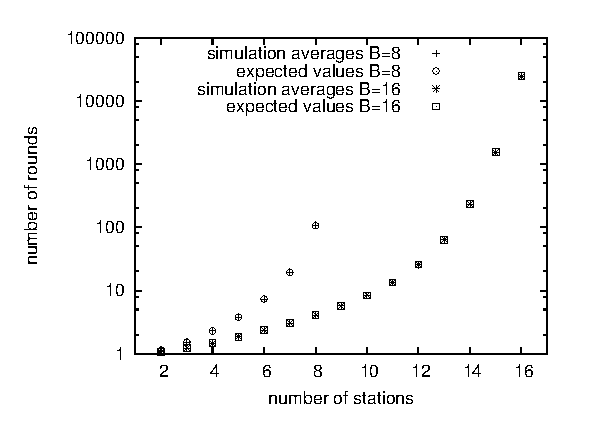
\includegraphics[height=6.2cm]{figures/convergence_avg}
\caption{The analytically computed expectation is compared to simulation averages. Two different values for $B$ have been considered ($B=8$ and $B=16$) and $N$ takes values from 2 to 16.}
\label{fig:convergence_avg}
\end{figure}


In this section we present simulation results that validate the expressions derived in the previous section.
The simulation scenario is exactly the one described in Sect. \ref{sec:markov_chain}.
The number of slots in each round is set to $B=8$ and $B=16$, and the number of contenders $N$ takes values from 2 to 16.
The contenders choose the same slot in the case of successful transmission and a random slot if the transmission is unsuccessful.

The first results are for an ideal channel that does not introduce errors.
We compare the analytically computed expected number of steps to absorption and the average number of steps to reach collision-free operation obtained from 10,000 executions of a custom simulator in c.\footnote{The two simulators in c that we have used and the scripts in maxima to compute the expectations derived from the analytical model can be downloaded from www.jaumebarcelo.info/papers/barcelo-macom2012-sources.zip .} 
The results are presented in Fig.~\ref{fig:convergence_avg}.

To compute the expected value of the number of steps to absorption, it is necessary to follow the steps described in \cite{grinstead1997ip}.
First we construct the matrix $\psi^{B,N}$ which is a square matrix of size $N+1$.
If we number the rows and columns starting with zero, the element in row $d$ and column $\delta$ is simply $\left[\psi^{B,N}\right]_{d,\delta} = \psi^{B,N}_{d,\delta}$ as in  (\ref{eq:psi}).
The first $N$ (from 0 to $N-1$) rows represent transitions from the transient states and the $N$-th row is the absorbing state.
The $\mathbf{Q}$ matrix is constructed taking the first $N$ rows and columns of $\psi^{B,N}$ and the fundamental matrix of the absorbing MC is $\mathbf{N}= (\mathbf{I}-\mathbf{Q})^{-1}$, where $\mathbf{I}$ is the identity matrix.
Then, the number of steps to absorption if the system starts in state $S_0$ is the first entry of a vector $\mathbf{t}$ computed as $\mathbf{t}=\mathbf{N}\mathbf{c}$, where $\mathbf{c}$ is a column vector of ones.

To offer further insight on the convergence process, we also compute the 5-th, 25-th, 50-th, 75-th and 95-th percentiles of the number of steps to absorption for the case $B=16$, which are presented in Fig.~\ref{fig:convergence_stats}.
These percentiles provide an idea of the distribution of the value of the number steps required to reach collision-free operation.
\begin{figure}[h]
\centering
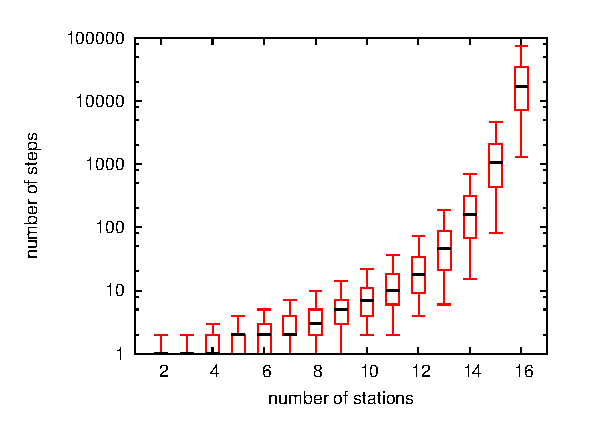
\includegraphics[height=6.2cm]{figures/convergence_stats}
\caption{The 5, 25, 50, 75, and 95 percentiles of the number of steps to convergence obtained from 10,000 simulation runs. $B=16$ and $N$ takes values from 2 to 16.}
\label{fig:convergence_stats}
\end{figure}


\subsection{Results in the presence of channel errors}
So far we have not considered the possibility that the channel introduced errors. 
In the case of channel error, a transmission will be unsuccessful even if it has not suffered a collision.
An erroneous transmission has the same effect of a collision and the station that suffered a channel error will randomly select its next transmission slot.

The probability of moving from the state $S_d$ to the state $S_\delta$ in the presence of a channel error probability $\epsilon$ is
\begin{equation}
\label{eq:psiBNepsilon}
\psi^{B,N,\epsilon}_{d,\delta}= \psi^{B,N}_{d,\delta} (1-\epsilon)^\delta + \sum_{i=\delta+1}^{N} \binom{i}{\delta} \epsilon^{i-\delta}(1-\epsilon)^\delta \psi^{B,N}_{d,i}.
\end{equation}

The probability that there are exactly $\delta$ successful stations is the probability that there are $\delta$ stations that do not collide and none of them suffers a collision plus the probability that there are $i$ ($\delta < i \leq N$) stations that do not collide and exactly $i-\delta$ of those stations suffer a collision.
Note that the resulting MC is no longer absorbing.
In this case, to validate the expression in (\ref{eq:psiBNepsilon}) we compute the average number of successful transmissions in each step from the MC and compare it with averages obtained from a simulation of 10,000 rounds.
The results for a channel error probability $\epsilon=0.1$, different numbers of slots ($B$) and different numbers of contenders ($N$) are presented in Fig.~\ref{fig:successful_tx_per_step}.

\begin{figure}[h]
\centering
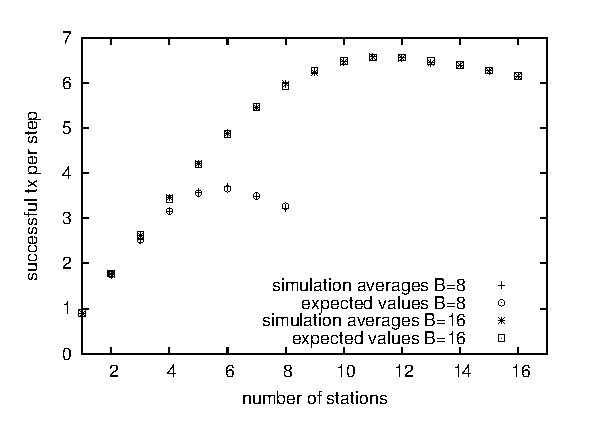
\includegraphics[height=6.2cm]{figures/successful_tx_per_step}
\caption{The average number of successful transmissions in every round obtained from simulation is compared to the analytically computed expected values.}
\label{fig:successful_tx_per_step}
\end{figure}

\section{Conclusion}
\label{sec:conclusion}

In this paper we have studied a Decentralized Constraint Satisfaction (DCS) problem solver to assign channel slots to contending stations.
The stations deterministically choose their transmission slots after successful transmissions.
If the transmission is not successful, the station randomly chooses its next transmission slot.
The system eventually converges to collision-free operation in ideal channel conditions.

We have modeled the convergence process as a MC and have derived closed expressions for the transition probabilities.
These values can be used to compute the expected number of steps required for the system to converge to a solution.

We have also considered the possibility of the presence of channel errors and constructed the MC that accounts for channel errors, which is no longer an absorbing MC.

The presented results have been validated by means of simulation.





% if have a single appendix:
%\appendix[Proof of the Zonklar Equations]
% or
%\appendix  % for no appendix heading
% do not use \section anymore after \appendix, only \section*
% is possibly needed

% use appendices with more than one appendix
% then use \section to start each appendix
% you must declare a \section before using any
% \subsection or using \label (\appendices by itself
% starts a section numbered zero.)
%


\appendices
\section{Proof of the First Zonklar Equation}
Appendix one text goes here.

% you can choose not to have a title for an appendix
% if you want by leaving the argument blank
\section{}
Appendix two text goes here.


% use section* for acknowledgement
\section*{Acknowledgment}


The authors would like to thank...


% Can use something like this to put references on a page
% by themselves when using endfloat and the captionsoff option.
\ifCLASSOPTIONcaptionsoff
  \newpage
\fi



% trigger a \newpage just before the given reference
% number - used to balance the columns on the last page
% adjust value as needed - may need to be readjusted if
% the document is modified later
%\IEEEtriggeratref{8}
% The "triggered" command can be changed if desired:
%\IEEEtriggercmd{\enlargethispage{-5in}}

% references section

% can use a bibliography generated by BibTeX as a .bbl file
% BibTeX documentation can be easily obtained at:
% http://www.ctan.org/tex-archive/biblio/bibtex/contrib/doc/
% The IEEEtran BibTeX style support page is at:
% http://www.michaelshell.org/tex/ieeetran/bibtex/
\bibliographystyle{IEEEtran}
% argument is your BibTeX string definitions and bibliography database(s)
\bibliography{IEEEabrv,my_bib}
%
% <OR> manually copy in the resultant .bbl file
% set second argument of \begin to the number of references
% (used to reserve space for the reference number labels box)
%\begin{thebibliography}{1}

%\bibitem{IEEEhowto:kopka}
%H.~Kopka and P.~W. Daly, \emph{A Guide to \LaTeX}, 3rd~ed.\hskip 1em plus
%  0.5em minus 0.4em\relax Harlow, England: Addison-Wesley, 1999.

%\end{thebibliography}

% biography section
% 
% If you have an EPS/PDF photo (graphicx package needed) extra braces are
% needed around the contents of the optional argument to biography to prevent
% the LaTeX parser from getting confused when it sees the complicated
% \includegraphics command within an optional argument. (You could create
% your own custom macro containing the \includegraphics command to make things
% simpler here.)
%\begin{biography}[{\includegraphics[width=1in,height=1.25in,clip,keepaspectratio]{mshell}}]{Michael Shell}
% or if you just want to reserve a space for a photo:

\begin{IEEEbiography}{Michael Shell}
Biography text here.
\end{IEEEbiography}

% if you will not have a photo at all:
\begin{IEEEbiographynophoto}{John Doe}
Biography text here.
\end{IEEEbiographynophoto}

% insert where needed to balance the two columns on the last page with
% biographies
%\newpage

\begin{IEEEbiographynophoto}{Jane Doe}
Biography text here.
\end{IEEEbiographynophoto}

% You can push biographies down or up by placing
% a \vfill before or after them. The appropriate
% use of \vfill depends on what kind of text is
% on the last page and whether or not the columns
% are being equalized.

%\vfill

% Can be used to pull up biographies so that the bottom of the last one
% is flush with the other column.
%\enlargethispage{-5in}



% that's all folks
\end{document}


